\section{Evaluation}

For performance analysis of the proposed solution, we evaluated a few most common graph algorithms using real-world sparse matrix data. 
As a baseline for comparison we chose LAGraph~\cite{szarnyas2021lagraph} in connection with SuiteSparse~\cite{10.1145/3322125} as a CPU tool, Gunrock~\cite{7967137} and GraphBLAST~\cite{yang2019graphblast} as a Nvidia GPU tools. 
Also, we tested algorithms on several devices with distinct OpenCL vendors in order to validate the portability of the proposed solution. 
In general, these evaluation intentions are summarized in the following research questions. 

\vspace{0.2cm}
\begin{itemize}
    \item[\textbf{RQ1}] What is the performance of the proposed solution relative to existing tools for GPU analysis?

    \item[\textbf{RQ2}] What is the performance of the proposed solution on various devices vendors and OpenCL runtimes?

    \item[\textbf{RQ3}] What is the performance of the proposed solution on integrated GPU compared to existing CPU tool for analysis?
\end{itemize}

\subsection{Evaluation Setup}

\textbf{For evaluation of RQ1}, we use a PC with Ubuntu 20.04 installed, which has 3.40Hz Intel Core i7-6700 4-core CPU, DDR4 64Gb RAM, Intel HD Graphics 530 integrated GPU, and Nvidia GeForce GTX 1070 dedicated GPU with 8Gb on-board VRAM. 
\textbf{For evaluation of RQ2}, we use a PC with Ubuntu 22.04 installed, which has 4.70Hz AMD Ryzen 9 7900x 12-core CPU, DDR4 128 GB RAM, AMD GFX1036 integrated GPU, and either Intel Arc A770 flux dedicated GPU with 8GB on-board VRAM or AMD Radeon Vega Frontier Edition dedicated GPU with 16GB on-board VRAM.
\textbf{For evaluation of RQ3}, the first PC with Intel CPU and integrated GPU and the second PC with AMD CPU and integrated GPU are used.

Programs using CUDA were compiled with GCC v8.4.0 and Nvidia NVCC v10.1.
Release mode and maximum optimization level were enabled for all tested programs. 
Data loading time, preparation, format transformations, and host-device initial communications are excluded from time measurements. 
All tests are averaged across 10 runs. The deviation of measurements does not exceed the threshold of 10 percent. Additional warm-up run for each test execution is excluded from measurements.

\subsection{Graph Algorithms}

For preliminary study \textit{breadth-first search} (BFS), \textit{single-source shortest paths} (SSSP), \textit{page rank} (PR) and \textit{triangles counting} (TC) algorithms were chosen.
Implementation of those algorithms is used from official examples packages of tested libraries with default parameters. Compared tools are allowed to make any optimizations as long as the result remains correct.
The graph vertex with index 1 is set as the initial traversal vertex in the algorithms BFS and SSSP for all tested instruments and all tested devices.

\subsection{Dataset}

Thirteen matrices with graph data were selected from the Sparse Matrix Collection at University of Florida~\cite{dataset:10.1145/2049662.2049663}. 
Information about graphs is summarized in Table~\ref{dataset:info}. 
The dataset is converted to undirected graphs. 
Self-loops and duplicated edges are removed. 
Average, sd and max metrics relate to out degree property of the vertices.
For SSSP weights are initialized using pseudo-random generator with uniform $[0, 1]$ distribution of floating-point values.

Graphs are roughly divided into two groups. 
The first group represents relatively dense graphs, where the number of edges per node is sufficient on average to effectively load the GPU with useful work. 
The second group represents relatively sparse graphs, where the average vertex degree is below the typical GPU vector register size, and the search depth reaches hundreds of hoops. 
Graphs are sorted in ascending order by the number of vertices within each group.

\begin{table}[tbp]
\caption{Dataset description.} 
\begin{center}
    \rowcolors{2}{black!2}{black!10}
    \begin{tabular}{|l|r|r|r|r|r|}
    \hline
    Graph&Vertices&Edges&Avg&Sd&Max\\
    \hline
    \hline
    coAuthorsCit&227.3K&1.6M&7.2&10.6&1.4K\\
    coPapersDBLP&540.5K&30.5M&56.4&66.2&3.3K\\
    amazon2008&735.3K&7.0M&9.6&7.6&1.1K\\
    hollywood2009&1.1M&112.8M&98.9&271.9&11.5K\\
    comOrkut&3.1M&234.4M&76.3&154.8&33.3K\\
    citPatents&3.8M&33.0M&8.8&10.5&793.0\\
    socLiveJournal&4.8M&85.7M&17.7&52.0&20.3K\\
    indochina2004&7.4M&302.0M&40.7&329.6&256.4K\\
    \hline
    belgiumosm&1.4M&3.1M&2.2&0.5&10.0\\
    roadNetCA&2.0M&5.5M&2.8&1.0&12.0\\
    rggn222s0&4.2M&60.7M&14.5&3.8&36.0\\
    rggn223s0&8.4M&127.0M&15.1&3.9&40.0\\
    roadcentral&14.1M&33.9M&2.4&0.9&8.0\\
    \hline
    \end{tabular}
    \label{dataset:info}
\end{center}
\end{table}

\subsection{Results Summary}

\begin{figure}[tbp]
\centering
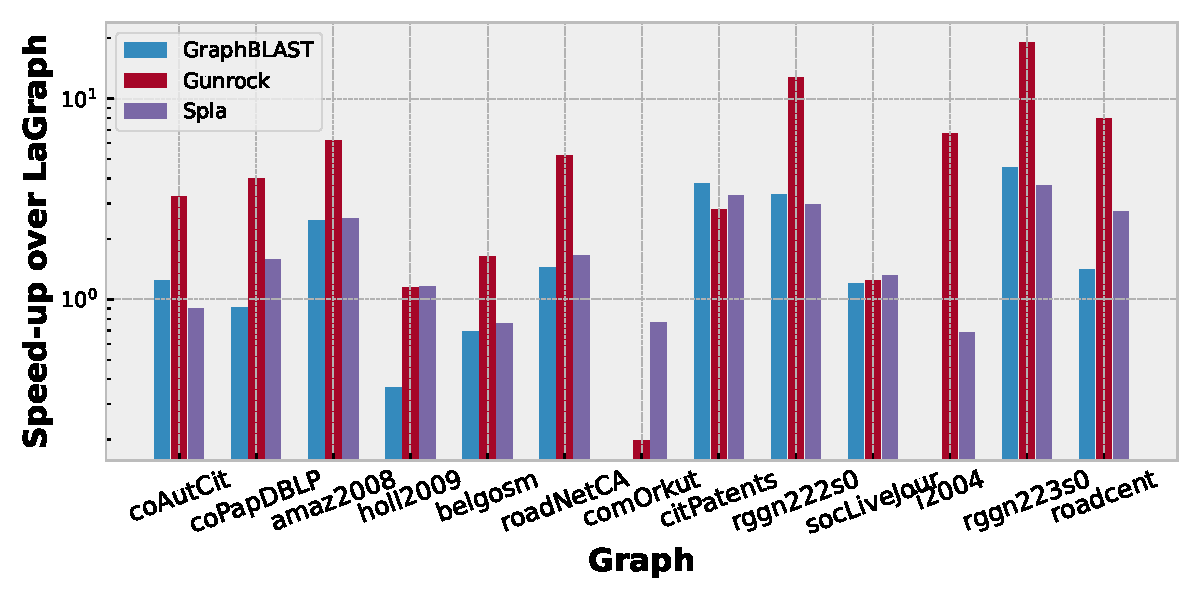
\includegraphics[width=0.9\linewidth]{plots/rq1_rel_bfs.pdf}
\caption{Performance of GPU tools in BFS algorithm compared to LaGraph. Logarithmic scale is used.}
\label{fig:rq1_bfs}
\end{figure}

\begin{figure}[tbp]
\centering
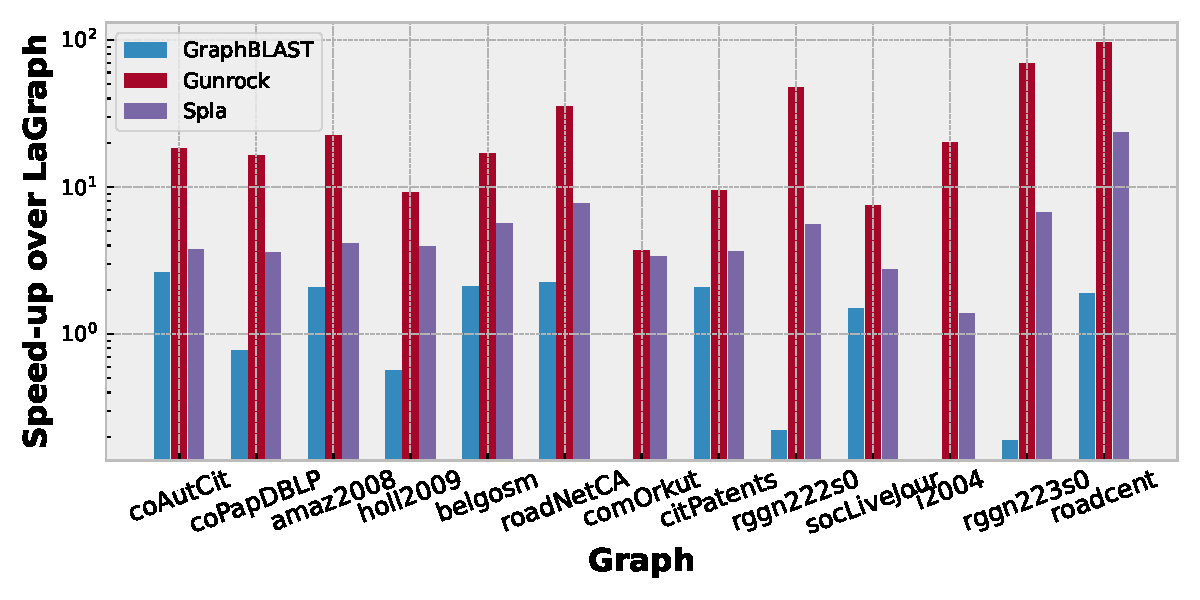
\includegraphics[width=0.9\linewidth]{plots/rq1_rel_sssp.pdf}
\caption{Performance of GPU tools in SSSP algorithm compared to LaGraph. Logarithmic scale is used.}
\label{fig:rq1_sssp}
\end{figure}

\begin{figure}[tbp]
\centering
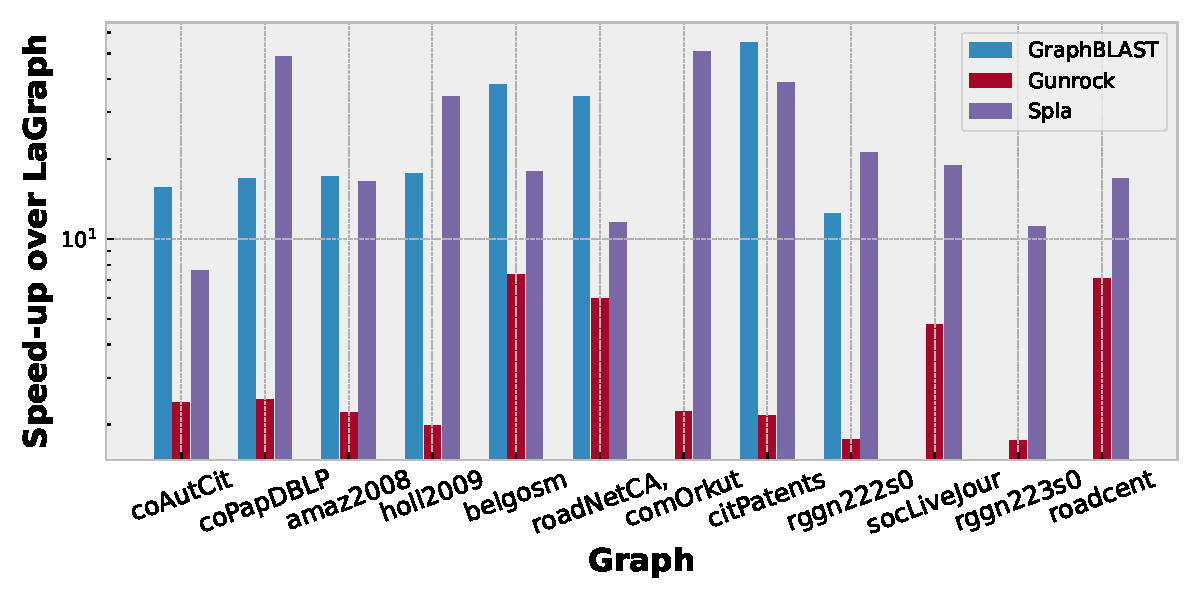
\includegraphics[width=0.9\linewidth]{plots/rq1_rel_pr.pdf}
\caption{Performance of GPU tools in PR algorithm compared to LaGraph. Logarithmic scale is used.}
\label{fig:rq1_pr}
\end{figure}

\begin{figure}[tbp]
\centering
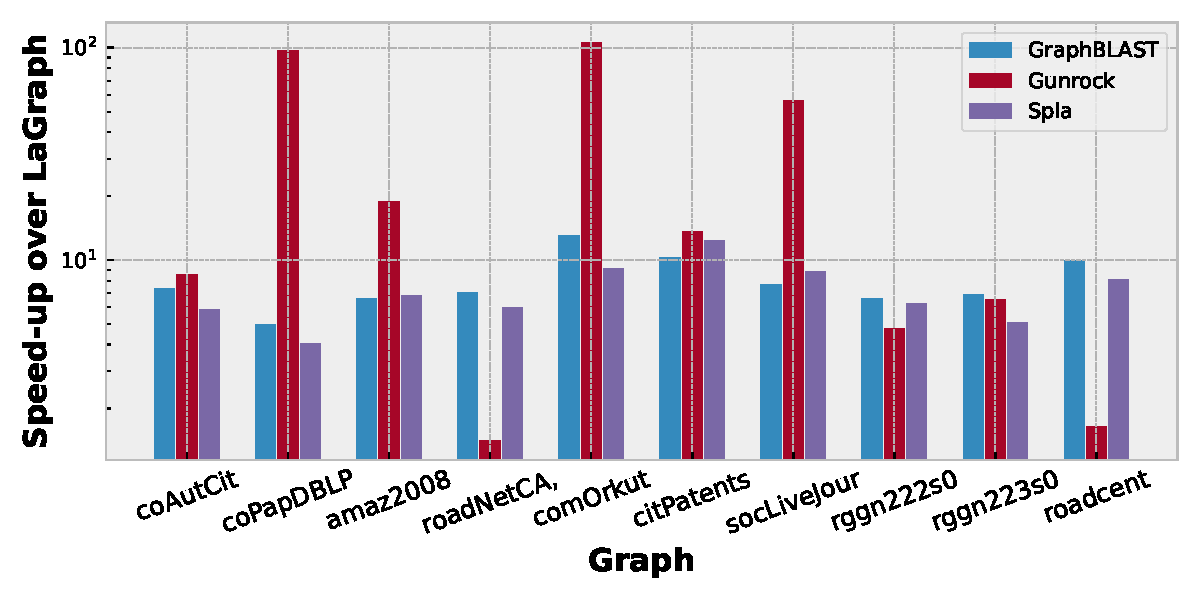
\includegraphics[width=0.9\linewidth]{plots/rq1_rel_tc.pdf}
\caption{Performance of GPU tools in TC algorithm compared to LaGraph. Logarithmic scale is used.}
\label{fig:rq1_tc}
\end{figure}


\begin{figure}[tbp]
\centering
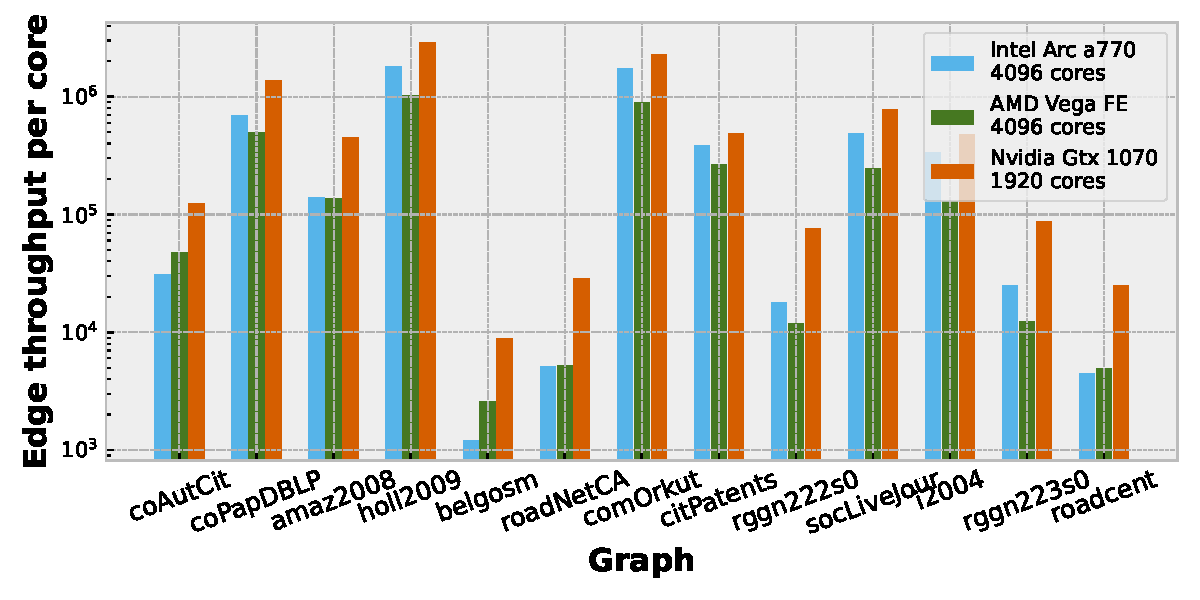
\includegraphics[width=0.9\linewidth]{plots/rq2_cores_bfs.pdf}
\caption{Performance of Spla library in BFS algorithm on different devices relative to number of compute cores. Logarithmic scale is used.}
\label{fig:rq2_bfs}
\end{figure}

\begin{figure}[tbp]
\centering
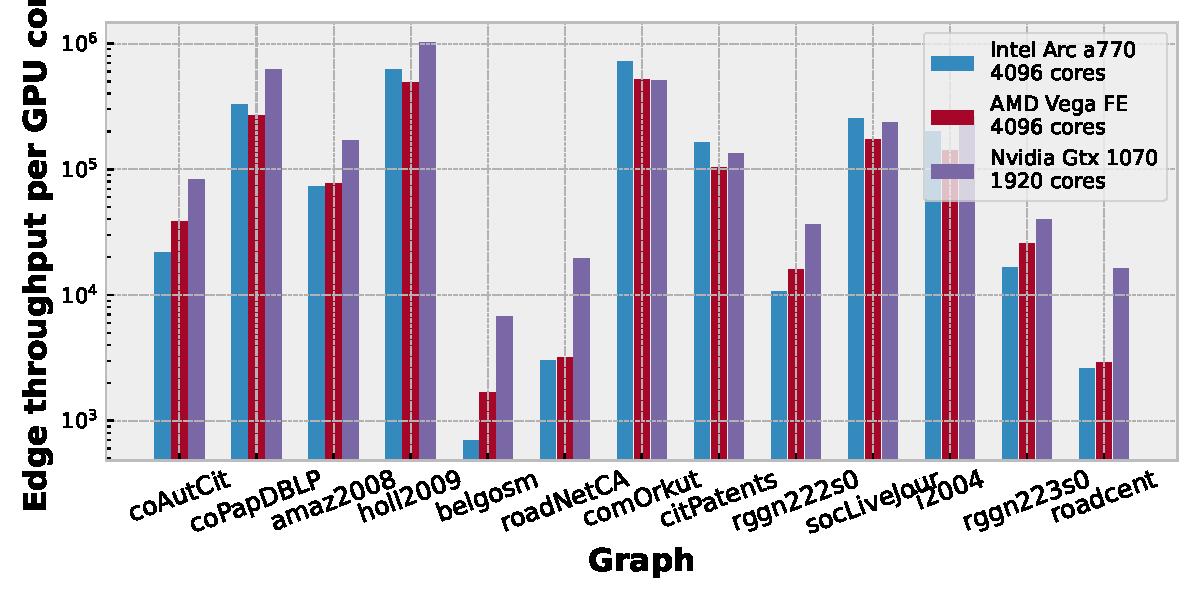
\includegraphics[width=0.9\linewidth]{plots/rq2_cores_sssp.pdf}
\caption{Performance of Spla library in SSSP algorithm on different devices relative to number of compute cores. Logarithmic scale is used.}
\label{fig:rq2_sssp}
\end{figure}

\begin{figure}[tbp]
\centering
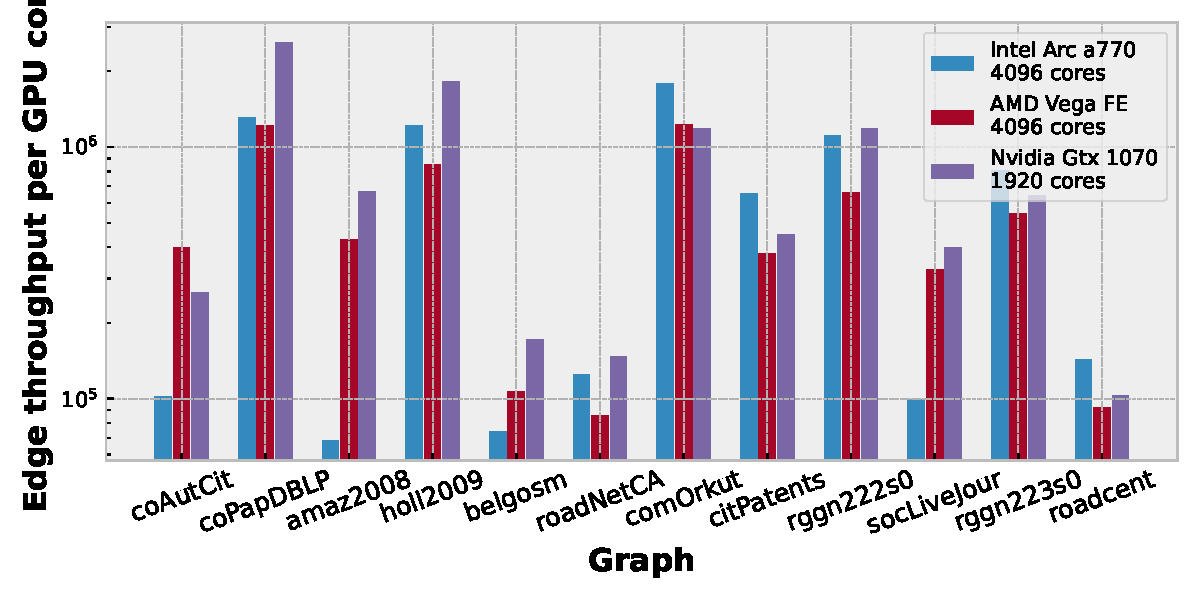
\includegraphics[width=0.9\linewidth]{plots/rq2_cores_pr.pdf}
\caption{Performance of Spla library in PR algorithm on different devices relative to number of compute cores. Logarithmic scale is used.}
\label{fig:rq2_pr}
\end{figure}

\begin{figure}[tbp]
\centering
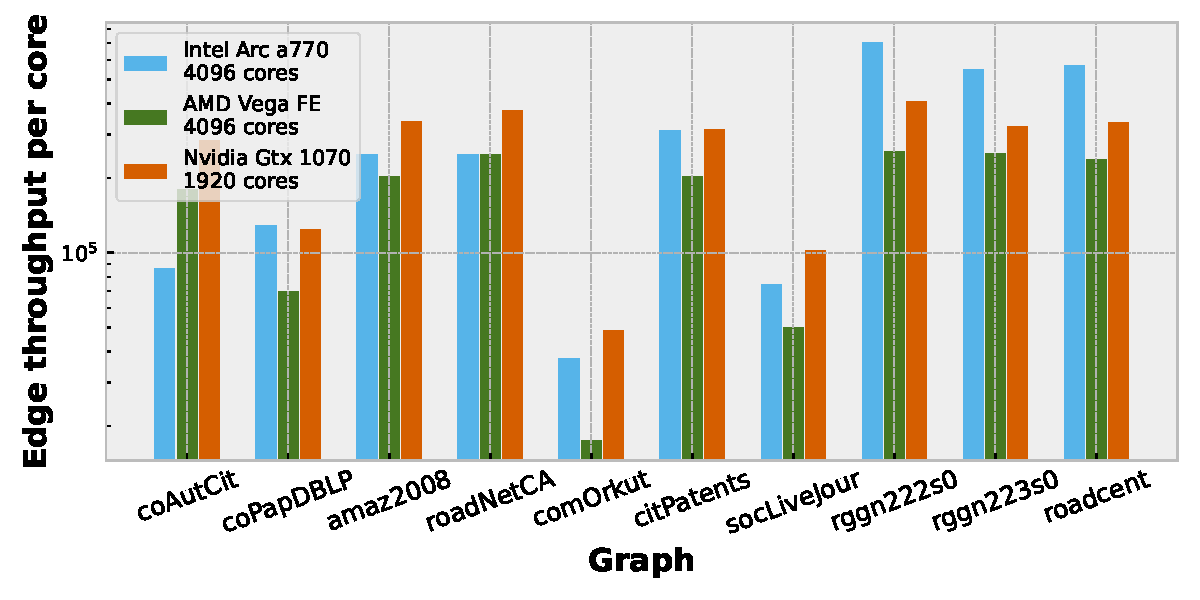
\includegraphics[width=0.9\linewidth]{plots/rq2_cores_tc.pdf}
\caption{Performance of Spla library in TC algorithm on different devices relative to number of compute cores. Logarithmic scale is used.}
\label{fig:rq2_tc}
\end{figure}


\begin{figure}[tbp]
\centering
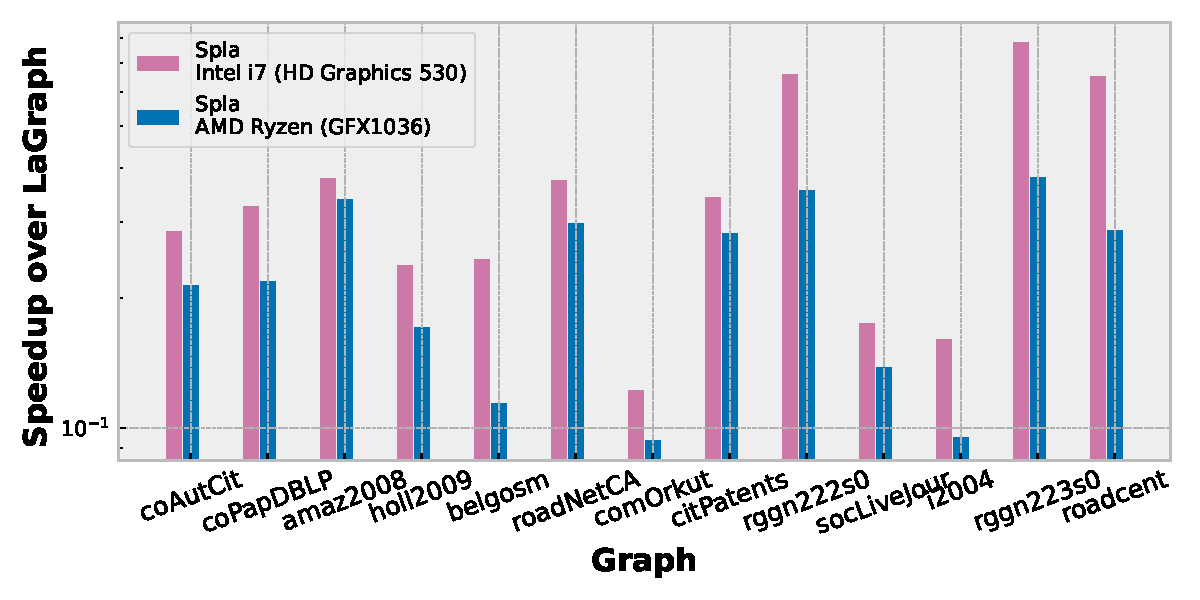
\includegraphics[width=0.9\linewidth]{plots/rq3_int_bfs.pdf}
\caption{Performance of Spla library in BFS on integrated GPU compared to LaGraph on the same chip. Logarithmic scale is used.}
\label{fig:rq3_bfs}
\end{figure}

\begin{figure}[tbp]
\centering
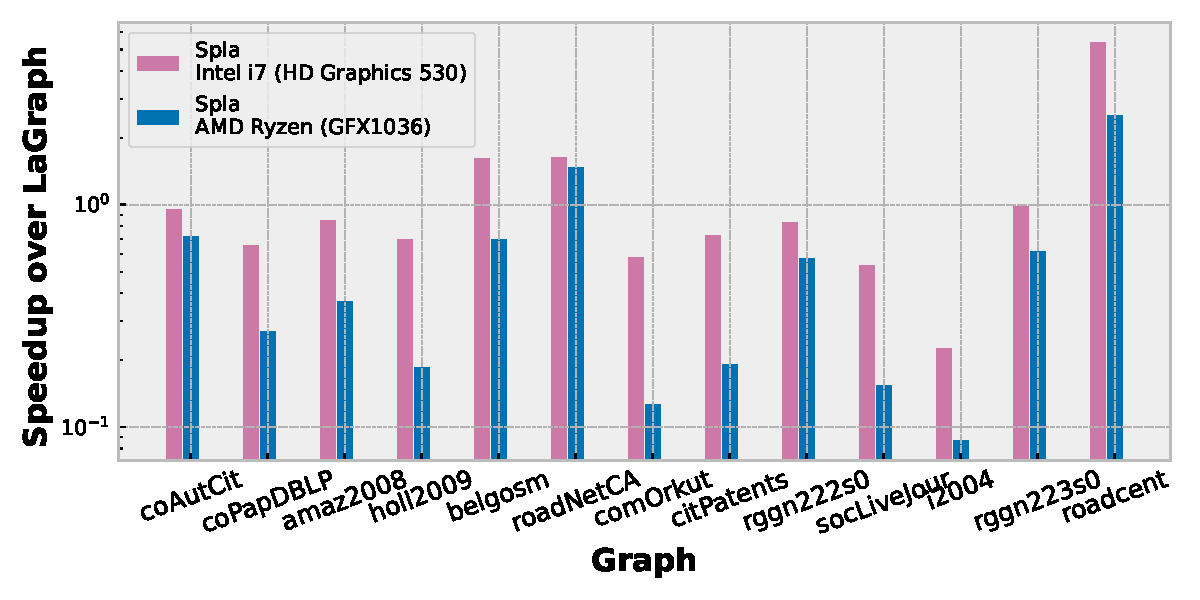
\includegraphics[width=0.9\linewidth]{plots/rq3_int_sssp.pdf}
\caption{Performance of Spla library in SSSP on integrated GPU compared to LaGraph on the same chip. Logarithmic scale is used.}
\label{fig:rq3_sssp}
\end{figure}

\begin{figure}[tbp]
\centering
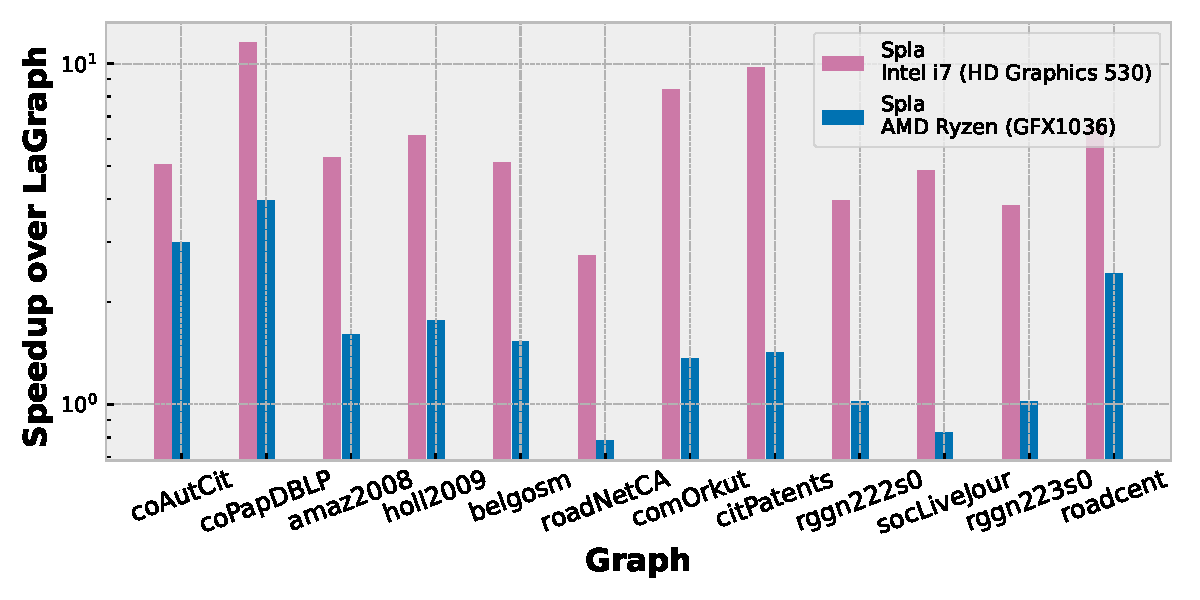
\includegraphics[width=0.9\linewidth]{plots/rq3_int_pr.pdf}
\caption{Performance of Spla library in PR on integrated GPU compared to LaGraph on the same chip. Logarithmic scale is used.}
\label{fig:rq3_pr}
\end{figure}

\begin{figure}[tbp]
\centering
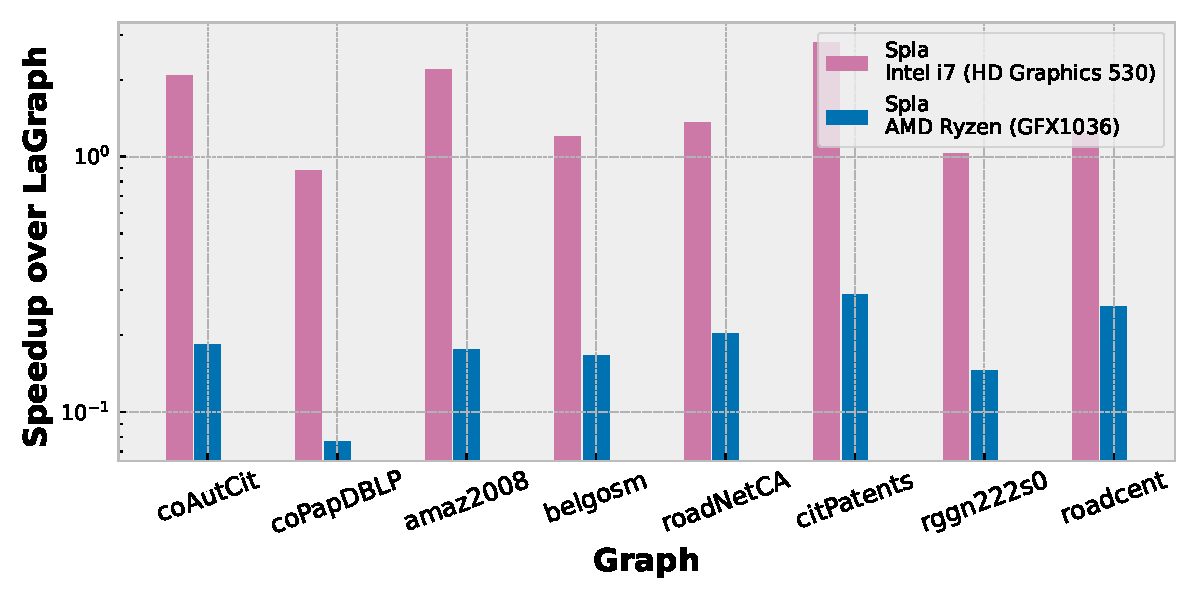
\includegraphics[width=0.9\linewidth]{plots/rq3_int_tc.pdf}
\caption{Performance of Spla library in TC on integrated GPU compared to LaGraph on the same chip. Logarithmic scale is used.}
\label{fig:rq3_tc}
\end{figure}

Table~\ref{rq1_table} presents results of the evaluation and compares the performance of Spla against other Nvidia GPU tools and uses as a baseline LaGraph CPU tool. 
Table~\ref{rq2_table} presents result of the portability analysis of the proposed solution. It shows performance of the proposed solution on discrete GPUs of distinct vendors.
Table~\ref{rq3_table} present result of per-device comparison of Spla library running on integrated GPU and CPU LaGraph running on the same chip.

Cell left empty with \textit{none} if tested tool failed to analyze graph due to \textit{out of memory} exception.\\

\textit{RQ1. What is the performance of the proposed solution relative to existing tools for GPU analysis?}\\

In general, Spla shows very acceptable performance in all algorithms, running with comparable speed to its nearest competitor, GraphBLAST. Also proposed library does not not suffer from memory issues on some large graphs such as indochina or orkut. Spla is consistently several times faster than LaGraph, overcoming it up to $12\times$ in some cases. Gunrock, the fastest GPU framework for analysis, dominates the overall performance and only suffers in a PR algorithm.

Taking a closer look at Fig.~\ref{fig:rq1_bfs}, Spla BFS shows comparable to GraphBLAST performance in most runs. Spla has good speed at relatively dense graphs with high vertex degree and small depth of the search, what allows to saturate GPU with a work better. However, the performance degrades in network and road graphs with small front of the search and large diameter, what cause a lot of iterations. Thus, both Spla and GraphBLAST suffer from the overhead of kernel launches and relatively small amount of the work for a GPU. SSSP in Fig.~\ref{fig:rq1_sssp} shares with BFS the same picture in general. However, Spla behaves here slightly better than GraphBLAST, running up to $36\times$ faster at some extreme cases.

For a PR in Fig.~\ref{fig:rq1_pr}, Spla and GraphBLAST show the best performance, except cases with GraphBLAST memory issues. Both tools are faster than Gunrock in average reaching up to $20\times$ and more relative speedup. This performance can be motivated by the usage of mxv operation as core primitive, which is computationally intensive and has good work load balance. Spla suffers a bit in case of lower-degree graphs due to lack of more precise balance for small matrix rows.

Finally, detailed TC results are shown in Fig.~\ref{fig:rq1_tc}. Gunrock dominates performance as well, except two sparse road graphs where it has significant performance drop down. Spla and GraphBLAST have comparable results. However, GraphBLAST slightly faster nearly in all runs. Both tools use the same approach for mxmT implementation. However, Spla may encounter some OpenCL overhead or lack of precise performance tuning.\\

\textit{RQ2. What is the performance of the proposed solution on various devices vendors and OpenCL runtimes?}\\

Spla successfully launches and workes on the GPU of distinct vendors, including Intel, AMD and Nvidia. It shows promising performance and demonstrated scalability in relation to the number of computing cores. Fig.~\ref{fig:rq2_bfs} for BFS, Fig.~\ref{fig:rq2_sssp} for SSSP, Fig.~\ref{fig:rq2_pr} and Fig.~\ref{fig:rq2_tc} depict the edge per second throughput per a GPU core for all devices. This metric is quite predictable for the same graphs. This can be seen if one takes into account the overall shape of the figures for BFS, SSSP and PR as a whole.

In general, Spla on Nvidia shows better average performance, especially for sparser graphs with smaller degree per row. Nvidia OpenCL driver features faster memory allocations and has less overhead on a frequent kernel launches. Spla on Intel runtime lags a bit behind Nvidia, but performs better on some TC runs as shown in Fig.~\ref{fig:rq2_tc}. Spla performance on AMD is acceptable. However, better tuning and further polishing are required.\\

\textit{RQ3. What is the performance of the proposed solution on integrated GPU compared to existing CPU tool for analysis?}\\

Result of detailed comparison are shown in Fig.~\ref{fig:rq3_bfs} for BFS, Fig.~\ref{fig:rq3_sssp} for SSSP, Fig.~\ref{fig:rq3_pr} for PR and Fig.~\ref{fig:rq3_tc} for TC. These figures depict Spla relative to LaGraph speedup on the same chip, where Spla is running on integrated GPU part and LaGraph is running on multi-core CPU part. 

In general, LaGraph shows better performance for both CPUs, especially on a new powerful AMD Ryzen with 12 cores. The difference in a speed is extremely dramatic in BFS and SSSP algorithms. For a PR algorithm the picture is slightly better. Spla shows up to $10\times$ speedup. PR algorithm tends to be more computationally intensive, so difference to BFS and SSSP is reasonable. For TC Spla performs better only for Intel device, having in some cases conservative $2\times$ speedup. 

\begin{table}[tbp]
\caption{Performance comparison of the proposed solution.\\Time in milliseconds (lower is better).} 
\begin{center}
    \begin{tabular}{|l|r|r|r|r|}
    \hline
    Dataset & GB & GR & LG & SP \\
    \hline
    \hline
    \multicolumn{5}{|c|}{BFS} \\
    \hline
    \rowcolor{black!10} coAuthorsCit&5.0&1.9&6.3&6.9\\
    \rowcolor{black!2 } coPapersDBLP&19.9&4.5&18.0&11.5\\
    \rowcolor{black!10} amazon2008&8.3&3.3&20.4&8.1\\
    \rowcolor{black!2 } hollywood2009&64.3&20.3&23.4&20.3\\
    \rowcolor{black!10} belgiumosm&200.6&84.4&138.0&181.2\\
    \rowcolor{black!2 } roadNetCA&116.3&32.4&168.2&101.7\\
    \rowcolor{black!10} comOrkut& none&205.0&40.6&53.2\\
    \rowcolor{black!2 } citPatents&30.6&41.3&115.9&35.1\\
    \rowcolor{black!10} rggn222s0&367.3&95.9&1228.1&415.3\\
    \rowcolor{black!2 } socLiveJournal&63.1&61.0&75.5&57.1\\
    \rowcolor{black!10} indochina2004& none&33.3&224.6&328.7\\
    \rowcolor{black!2 } rggn223s0&615.3&146.2&2790.0&754.9\\
    \rowcolor{black!10} roadcentral&1383.4&243.8&1951.0&710.2\\
    \hline
    \hline
    \multicolumn{5}{|c|}{SSSP} \\
    \hline
    \rowcolor{black!10} coAuthorsCit&14.7&2.1&38.9&10.3\\
    \rowcolor{black!2 } coPapersDBLP&118.6&5.6&92.2&25.7\\
    \rowcolor{black!10} amazon2008&43.4&4.0&90.0&21.7\\
    \rowcolor{black!2 } hollywood2009&404.3&24.6&227.7&57.5\\
    \rowcolor{black!10} belgiumosm&650.2&81.1&1359.8&240.9\\
    \rowcolor{black!2 } roadNetCA&509.7&32.4&1149.3&147.9\\
    \rowcolor{black!10} comOrkut& none&219.0&806.5&241.0\\
    \rowcolor{black!2 } citPatents&226.9&49.8&468.5&129.3\\
    \rowcolor{black!10} rggn222s0&21737.8&101.9&4808.8&865.4\\
    \rowcolor{black!2 } socLiveJournal&346.4&69.2&518.0&189.5\\
    \rowcolor{black!10} indochina2004& none&40.8&821.9&596.6\\
    \rowcolor{black!2 } rggn223s0&59015.7&161.1&11149.9&1654.8\\
    \rowcolor{black!10} roadcentral&13724.8&267.0&25703.4&1094.3\\
    \hline
    \hline
    \multicolumn{5}{|c|}{PR} \\
    \hline
    \rowcolor{black!10} coAuthorsCit&1.6&10.0&24.3&3.2\\
    \rowcolor{black!2 } coPapersDBLP&17.6&120.2&297.6&6.1\\
    \rowcolor{black!10} amazon2008&5.2&40.6&89.8&5.5\\
    \rowcolor{black!2 } hollywood2009&62.9&559.5&1111.2&32.4\\
    \rowcolor{black!10} belgiumosm&4.4&22.9&167.6&9.4\\
    \rowcolor{black!2 } roadNetCA&6.6&37.7&225.8&19.6\\
    \rowcolor{black!10} comOrkut& none&2333.6&5239.0&103.3\\
    \rowcolor{black!2 } citPatents&27.0&686.1&1487.0&38.3\\
    \rowcolor{black!10} rggn222s0&45.2&320.0&563.5&26.6\\
    \rowcolor{black!2 } socLiveJournal& none&445.9&2122.5&112.0\\
    \rowcolor{black!10} rggn223s0& none&662.7&1155.6&103.4\\
    \rowcolor{black!2 } roadcentral& none&408.8&2899.9&172.0\\
    \hline
    \hline
    \multicolumn{5}{|c|}{TC} \\
    \hline
    \rowcolor{black!10} coAuthorsCit&2.3&2.0&17.3&3.0\\
    \rowcolor{black!2 } coPapersDBLP&105.2&5.3&520.8&128.4\\
    \rowcolor{black!10} amazon2008&11.2&3.9&73.9&10.8\\
    \rowcolor{black!2 } roadNetCA&6.5&32.4&46.0&7.7\\
    \rowcolor{black!10} comOrkut&1776.9&218.0&23103.8&2522.0\\
    \rowcolor{black!2 } citPatents&65.5&49.7&675.0&54.5\\
    \rowcolor{black!10} socLiveJournal&504.3&69.2&3886.7&437.8\\
    \rowcolor{black!2 } rggn222s0&73.2&101.3&484.5&77.7\\
    \rowcolor{black!10} rggn223s0&151.4&158.9&1040.1&204.2\\
    \rowcolor{black!2 } roadcentral&42.6&259.3&425.3&52.7\\
    \hline
    \hline
    \multicolumn{5}{l}{GraphBLAST (GB), Gunrock (GR), LaGraph (LG), Spla (SP).} \\
    \end{tabular}
    \label{rq1_table}
\end{center}
\end{table}

\begin{table}[tbp]
\caption{Portability of the proposed solution.\\Time in milliseconds (lower is better).} 
\begin{center}
    \begin{tabular}{|l|r|r|r|}
    \hline
    Dataset & Intel Arc & AMD Vega & Nvidia Gtx\\
    \hline
    \hline
    \multicolumn{4}{|c|}{BFS} \\
    \hline
    \rowcolor{black!10} coAuthorsCit&12.8&8.3&6.9\\
    \rowcolor{black!2 } coPapersDBLP&10.8&14.9&11.5\\
    \rowcolor{black!10} amazon2008&12.3&12.6&8.1\\
    \rowcolor{black!2 } hollywood2009&15.3&26.7&20.3\\
    \rowcolor{black!10} belgiumosm&627.5&292.4&181.2\\
    \rowcolor{black!2 } roadNetCA&265.5&259.8&101.7\\
    \rowcolor{black!10} comOrkut&33.2&63.6&53.2\\
    \rowcolor{black!2 } citPatents&21.0&30.3&35.1\\
    \rowcolor{black!10} rggn222s0&825.3&1259.7&415.3\\
    \rowcolor{black!2 } socLiveJournal&43.0&85.8&57.1\\
    \rowcolor{black!10} indochina2004&220.6&573.4&328.7\\
    \rowcolor{black!2 } rggn223s0&1245.5&2519.6&754.9\\
    \rowcolor{black!10} roadcentral&1864.9&1680.8&710.2\\
    \hline
    \hline
    \multicolumn{4}{|c|}{SSSP} \\
    \hline
    \rowcolor{black!10} coAuthorsCit&18.3&10.4&10.3\\
    \rowcolor{black!2 } coPapersDBLP&22.9&27.7&25.7\\
    \rowcolor{black!10} amazon2008&23.4&22.2&21.7\\
    \rowcolor{black!2 } hollywood2009&44.6&56.2&57.5\\
    \rowcolor{black!10} belgiumosm&1085.9&454.8&240.9\\
    \rowcolor{black!2 } roadNetCA&447.3&422.5&147.9\\
    \rowcolor{black!10} comOrkut&79.7&111.5&241.0\\
    \rowcolor{black!2 } citPatents&49.8&78.4&129.3\\
    \rowcolor{black!10} rggn222s0&1378.8&924.3&865.4\\
    \rowcolor{black!2 } socLiveJournal&82.7&120.7&189.5\\
    \rowcolor{black!10} indochina2004&366.2&519.0&596.6\\
    \rowcolor{black!2 } rggn223s0&1880.2&1201.4&1654.8\\
    \rowcolor{black!10} roadcentral&3176.3&2848.8&1094.3\\
    \hline
    \hline
    \multicolumn{4}{|c|}{PR} \\
    \hline
    \rowcolor{black!10} coAuthorsCit&3.9&1.0&3.2\\
    \rowcolor{black!2 } coPapersDBLP&5.7&6.1&6.1\\
    \rowcolor{black!10} amazon2008&25.2&4.0&5.5\\
    \rowcolor{black!2 } hollywood2009&22.6&32.4&32.4\\
    \rowcolor{black!10} belgiumosm&10.2&7.1&9.4\\
    \rowcolor{black!2 } roadNetCA&10.8&15.7&19.6\\
    \rowcolor{black!10} comOrkut&31.9&46.6&103.3\\
    \rowcolor{black!2 } citPatents&12.3&21.3&38.3\\
    \rowcolor{black!10} rggn222s0&13.4&22.4&26.6\\
    \rowcolor{black!2 } socLiveJournal&210.0&64.2&112.0\\
    \rowcolor{black!10} rggn223s0&38.6&57.2&103.4\\
    \rowcolor{black!2 } roadcentral&57.9&89.6&172.0\\
    \hline
    \hline
    \multicolumn{4}{|c|}{TC} \\
    \hline
    \rowcolor{black!10} coAuthorsCit&4.6&2.2&3.0\\
    \rowcolor{black!2 } coPapersDBLP&57.6&106.2&128.4\\
    \rowcolor{black!10} amazon2008&6.9&8.5&10.8\\
    \rowcolor{black!2 } roadNetCA&5.4&5.4&7.7\\
    \rowcolor{black!10} comOrkut&1533.5&3267.6&2522.0\\
    \rowcolor{black!2 } citPatents&25.9&39.8&54.5\\
    \rowcolor{black!10} socLiveJournal&280.6&420.3&437.8\\
    \rowcolor{black!2 } rggn222s0&21.0&57.8&77.7\\
    \rowcolor{black!10} rggn223s0&56.7&123.2&204.2\\
    \rowcolor{black!2 } roadcentral&14.5&34.6&52.7\\
    \hline
    \hline
    \multicolumn{4}{l}{Distinct devices. Performance in not for comparison.} \\
    \end{tabular}
    \label{rq2_table}
\end{center}
\end{table}

\begin{table}[tbp]
\caption{Integrated GPU mode performance comparison of the proposed solution. Time in milliseconds (lower is better).} 
\begin{center}
    \begin{tabular}{|l|r|r|r|r|}
    \hline
    \multirow{2}{*}{Dataset} & \multicolumn{2}{c|}{Intel} & \multicolumn{2}{c|}{AMD} \\
    \cline{2-5}
    & LG & SP & LG & SP \\
    \hline
    \hline
    \multicolumn{5}{|c|}{BFS} \\
    \hline
    \rowcolor{black!10} coAuthorsCit&7.5&26.3&3.9&18.2\\
    \rowcolor{black!2 } coPapersDBLP&18.7&57.3&12.0&54.9\\
    \rowcolor{black!10} amazon2008&24.6&65.0&13.5&40.0\\
    \rowcolor{black!2 } hollywood2009&23.8&100.1&14.8&86.6\\
    \rowcolor{black!10} belgiumosm&131.4&536.0&60.0&527.6\\
    \rowcolor{black!2 } roadNetCA&173.2&461.8&100.8&339.7\\
    \rowcolor{black!10} comOrkut&41.6&341.4&25.2&269.4\\
    \rowcolor{black!2 } citPatents&126.9&371.6&61.3&217.7\\
    \rowcolor{black!10} rggn222s0&1288.0&1959.9&644.6&1821.7\\
    \rowcolor{black!2 } socLiveJournal&75.0&429.8&41.6&301.6\\
    \rowcolor{black!10} indochina2004&228.5&1424.8&137.0&1445.1\\
    \rowcolor{black!2 } rggn223s0&2850.8&3647.2&1403.9&3701.3\\
    \rowcolor{black!10} roadcentral&2087.8&3196.3&767.2&2670.3\\
    \hline
    \hline
    \multicolumn{5}{|c|}{SSSP} \\
    \hline
    \rowcolor{black!10} coAuthorsCit&40.5&42.5&29.2&40.5\\
    \rowcolor{black!2 } coPapersDBLP&92.9&141.8&48.9&181.6\\
    \rowcolor{black!10} amazon2008&97.4&114.4&48.3&131.3\\
    \rowcolor{black!2 } hollywood2009&236.7&337.9&93.8&507.4\\
    \rowcolor{black!10} belgiumosm&1383.2&854.3&588.9&845.7\\
    \rowcolor{black!2 } roadNetCA&1174.2&721.7&712.7&482.9\\
    \rowcolor{black!10} comOrkut&822.9&1420.5&214.8&1699.5\\
    \rowcolor{black!2 } citPatents&488.3&669.4&171.4&897.3\\
    \rowcolor{black!10} rggn222s0&4919.1&5928.3&2845.6&4952.9\\
    \rowcolor{black!2 } socLiveJournal&534.7&1007.7&185.3&1205.1\\
    \rowcolor{black!10} indochina2004&837.1&3708.3&345.5&3971.8\\
    \rowcolor{black!2 } rggn223s0&11375.6&11567.8&6099.6&9899.7\\
    \rowcolor{black!10} roadcentral&26314.1&4887.0&7867.2&3102.0\\
    \hline
    \hline
    \multicolumn{5}{|c|}{PR} \\
    \hline
    \rowcolor{black!10} coAuthorsCit&25.3&5.0&17.6&5.9\\
    \rowcolor{black!2 } coPapersDBLP&302.3&26.2&154.5&39.0\\
    \rowcolor{black!10} amazon2008&93.0&17.5&36.0&22.4\\
    \rowcolor{black!2 } hollywood2009&1109.8&179.9&531.7&300.7\\
    \rowcolor{black!10} belgiumosm&178.9&35.0&45.1&29.4\\
    \rowcolor{black!2 } roadNetCA&236.9&86.9&67.6&86.2\\
    \rowcolor{black!10} comOrkut&4458.5&531.9&959.6&701.4\\
    \rowcolor{black!2 } citPatents&1559.9&159.8&277.4&195.7\\
    \rowcolor{black!10} rggn222s0&576.7&145.9&275.1&270.2\\
    \rowcolor{black!2 } socLiveJournal&2181.0&449.7&520.5&630.9\\
    \rowcolor{black!10} rggn223s0&1187.0&309.3&617.2&605.3\\
    \rowcolor{black!2 } roadcentral&2995.8&461.4&993.7&409.8\\
    \hline
    \hline
    \multicolumn{5}{|c|}{TC} \\
    \hline
    \rowcolor{black!10} coAuthorsCit&17.3&8.3&5.2&28.3\\
    \rowcolor{black!2 } coPapersDBLP&534.1&604.2&129.4&1682.3\\
    \rowcolor{black!10} amazon2008&75.4&34.5&22.2&126.6\\
    \rowcolor{black!2 } belgiumosm&28.1&23.4&11.3&67.8\\
    \rowcolor{black!10} roadNetCA&47.7&35.2&21.5&105.6\\
    \rowcolor{black!2 } citPatents&693.1&247.6&170.5&589.3\\
    \rowcolor{black!10} rggn222s0&495.2&481.3&177.7&1218.1\\
    \rowcolor{black!2 } roadcentral&438.8&355.8&176.6&679.7\\
    \hline
    \hline
    \multicolumn{5}{l}{LaGraph (LG), Spla (SP).} \\
    \end{tabular}
    \label{rq3_table}
\end{center}
\end{table}




